% =======================
% LLM Application Evaluation Section
% =======================
\section{LLM Application Evaluation}

% ---------------- Slide: LLM Capabilities ----------------
\begin{frame}{What Can LLMs Do?}
\begin{columns}[T]
\begin{column}{0.48\textwidth}
\textbf{Core Capabilities:}
\begin{itemize}
  \item \textbf{Summarization} -- Condense documents
  \item \textbf{Generation} -- Create new content
  \item \textbf{Classification} -- Categorize inputs
  \item \textbf{Translation} -- Cross-language conversion
  \item \textbf{Extraction} -- Structured data from text
\end{itemize}
\end{column}
\begin{column}{0.48\textwidth}
\textbf{Evaluation Challenge:}
\begin{itemize}
  \item Output is \textbf{free-form text}
  \item Multiple valid answers exist
  \item ``Correctness'' is often subjective
  \item Traditional accuracy doesn't apply
\end{itemize}
\end{column}
\end{columns}

\begin{block}{Key Insight}
Unlike classification (one correct label), LLM outputs require \textbf{semantic} evaluation.
\end{block}
\end{frame}

% ---------------- Slide: Stochastic Nature ----------------
\begin{frame}{LLMs: A Distributional View}
\begin{itemize}
  \item Output is a \textbf{stochastic token trajectory}, not a single label
  \item Multiple completions can be acceptable for the same prompt
  \item Decoding parameters (temperature, top-p) change behavior
\end{itemize}

\begin{block}{Generative Process}
$$
P(y_1, y_2, \ldots, y_n \mid x) = \prod_{t=1}^{n} P(y_t \mid y_{<t}, x)
$$
where $y_{<t}$ are all tokens before position $t$.
\end{block}

\begin{tabular}{p{3cm}p{7cm}}
\toprule
\textbf{Control Point} & \textbf{Description} \\
\midrule
Model Choice & Claude, GPT, Llama, Nova, Gemini, etc. \\
Reasoning Mode & Enable/disable extended thinking (CoT) \\
Parameters & Temperature, top-p, max tokens \\
\textbf{Prompt} & \textbf{Most impactful lever} \\
\quad -- Static & System instructions, persona, rules \\
\quad -- Dynamic & User input, retrieved context \\
\bottomrule
\end{tabular}

\begin{block}{Key Insight}
Prompt engineering is often more impactful than model selection for task performance.
\end{block}
\end{frame}

% ---------------- Slide: Prompt Engineering ----------------
\begin{frame}{Prompt Engineering Strategies}

\begin{columns}[T]
\begin{column}{0.48\textwidth}
\textbf{Core Techniques:}
\begin{enumerate}
  \item \textbf{Clear Instructions} \\
        Explicit output format, constraints
  \item \textbf{Chain-of-Thought (CoT)} \\
        ``Think step by step...''
  \item \textbf{Few-Shot Examples} \\
        Provide input/output pairs
  \item \textbf{Role/Persona} \\
        ``You are an expert in...''
\end{enumerate}
\end{column}
\begin{column}{0.48\textwidth}
\textbf{Advanced Techniques:}
\begin{enumerate}
  \item \textbf{Self-Consistency} \\
        Sample multiple, take majority
  \item \textbf{Decomposition} \\
        Break complex tasks into steps
  \item \textbf{Guardrails} \\
        Define boundaries, edge cases
  \item \textbf{Abstention Prompting} \\
        Allow ``I don't know'' (next slide)
\end{enumerate}
\end{column}
\end{columns}

\vspace{0.5em}
\begin{block}{Evaluation Implication}
Each prompt version is a ``model'' that must be evaluated systematically.
\end{block}
\end{frame}

% ---------------- Slide: Abstention ----------------
\begin{frame}{Abstention: Trading Coverage for Accuracy}

\textbf{Problem:} LLMs have a bias toward producing answers even when uncertain.

\begin{block}{Abstention Prompting (``Unable to Classify'')}
Explicitly instruct the model to decline when information is insufficient:
\begin{quote}
\textit{``If the input lacks sufficient information about [X, Y, Z], respond with `Unable to determine' rather than guessing.''}
\end{quote}
\end{block}

\begin{columns}[T]
\begin{column}{0.48\textwidth}
\textbf{Without Abstention:}
\begin{itemize}
  \item High coverage
  \item Lower precision
  \item Hidden errors
\end{itemize}
\end{column}
\begin{column}{0.48\textwidth}
\textbf{With Abstention:}
\begin{itemize}
  \item Lower coverage
  \item Higher precision
  \item Explicit uncertainty
\end{itemize}
\end{column}
\end{columns}

\vspace{0.3em}
\begin{block}{When to Use}
Use abstention when the \textbf{cost of a wrong answer} exceeds the \textbf{cost of no answer}.
\end{block}
\end{frame}

% ---------------- Slide: Overfitting in Prompts ----------------
\begin{frame}{Avoiding Overfitting in Prompt Engineering}

\textbf{Key Insight:} Prompts can overfit to evaluation data, just like ML models.

\begin{block}{The Problem}
\begin{itemize}
  \item Developer iterates prompt on a fixed set of examples
  \item Prompt becomes highly tuned to those specific cases
  \item Performance degrades on unseen production data
\end{itemize}
\end{block}

\begin{block}{Best Practices}
\begin{enumerate}
  \item \textbf{Train/Test Split}: Calibrate prompt on one set, evaluate on held-out set
  \item \textbf{Stratified Sampling}: Ensure test set covers diverse input types
  \item \textbf{Version Control}: Track all prompt iterations and their metrics
  \item \textbf{Production Monitoring}: Compare offline metrics to online performance
\end{enumerate}
\end{block}

\begin{block}{Analogy to ML}
Prompt = Model, Examples in Prompt = Training Data, Evaluation Set = Test Set
\end{block}
\end{frame}

% ---------------- Slide: LLM Evaluation Toolkit ----------------
\begin{frame}{LLM Evaluation Toolkit}

\begin{enumerate}
  \item \textbf{Rubric-based Human Evaluation}
  \begin{itemize}
    \item Dimensions: correctness, completeness, safety, format, helpfulness
    \item Gold standard but expensive and slow
  \end{itemize}
  
  \item \textbf{Task-Specific Metrics}
  \begin{itemize}
    \item Extraction: accuracy, F1 on entities
    \item Classification: precision, recall, confusion matrix
    \item Code: execution success, test pass rate
    \item Structured output: schema validity
  \end{itemize}
  
  \item \textbf{LLM-as-a-Judge}
  \begin{itemize}
    \item Use a (often stronger) LLM to score outputs
    \item Scalable but requires calibration against human labels
    \item Must monitor for judge drift over time
  \end{itemize}
\end{enumerate}

\begin{block}{Key Principle}
Match evaluation method to \textbf{task risk} and \textbf{output structure}.
\end{block}
\end{frame}

% ---------------- Slide: Offline Workflow ----------------
\begin{frame}{Offline Evaluation Workflow}

\begin{center}
\begin{tikzpicture}[node distance=1.2cm, auto,
  block/.style={rectangle, draw, rounded corners, minimum height=0.8cm, minimum width=2.5cm, align=center, font=\small},
  arrow/.style={->, thick}
]
% Fallback: use description if tikz unavailable
\end{tikzpicture}
\end{center}

\textbf{Step-by-Step Process:}
\begin{enumerate}
  \item \textbf{Create Evaluation Dataset}
  \begin{itemize}
    \item Diverse inputs: typical cases, edge cases, adversarial examples
    \item Ground truth labels from domain experts (SMEs)
  \end{itemize}
  \item \textbf{Run Model/Prompt on Held-Out Test Set}
  \item \textbf{Compute Metrics} (task-appropriate)
  \item \textbf{If metrics meet threshold} $\rightarrow$ Deploy
  \item \textbf{If not} $\rightarrow$ Iterate on prompt, model, or architecture
\end{enumerate}

\begin{block}{Critical}
Test on \textbf{unseen data} to avoid prompt overfitting.
\end{block}
\end{frame}

% ---------------- Slide: Classification Case Study ----------------
\begin{frame}{Case Study: LLM for Hierarchical Classification}

\textbf{Task:} Multi-level decision tree classification (e.g., incident triage, document routing)

\begin{columns}[T]
\begin{column}{0.55\textwidth}
\textbf{Approach:}
\begin{itemize}
  \item Prompt-guided LLM navigates hierarchy top-to-leaf
  \item Chain-of-thought reasoning at each node
  \item Abstention when evidence insufficient
\end{itemize}

\textbf{Why GenAI over Traditional ML?}
\begin{itemize}
  \item No labeled training data required
  \item Native explainability (reasoning trace)
  \item Faster iteration (days vs. weeks)
  \item Handles semantic nuance
\end{itemize}
\end{column}
\begin{column}{0.42\textwidth}
\begin{center}
\footnotesize
\textbf{Decision Tree Example:}

\vspace{0.5em}
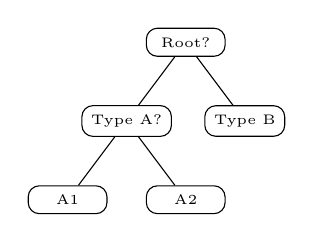
\begin{tikzpicture}[level distance=1cm, sibling distance=1.5cm,
  every node/.style={draw, rounded corners, font=\tiny, minimum width=1cm}]
  \node {Root?}
    child {node {Type A?}
      child {node {A1}}
      child {node {A2}}
    }
    child {node {Type B}};
\end{tikzpicture}
\end{center}
\end{column}
\end{columns}

\begin{block}{Key Insight}
This ``LLM app'' borrows heavily from \textbf{ML-style evaluation rigor}.
\end{block}
\end{frame}

% ---------------- Slide: Classification Metrics ----------------
\begin{frame}{Classification Metrics for LLM Applications}

When LLMs perform \textbf{structured tasks} (classification, extraction), use standard ML metrics:

\begin{columns}[T]
\begin{column}{0.48\textwidth}
\textbf{Core Metrics:}
\begin{itemize}
  \item \textbf{Accuracy}: $\frac{TP + TN}{Total}$
  \item \textbf{Precision}: $\frac{TP}{TP + FP}$
  \item \textbf{Recall}: $\frac{TP}{TP + FN}$
  \item \textbf{F1 Score}: Harmonic mean
\end{itemize}
\end{column}
\begin{column}{0.48\textwidth}
\textbf{When Costs are Asymmetric:}
\begin{itemize}
  \item If FN is costly $\rightarrow$ optimize \textbf{Recall}
  \item If FP is costly $\rightarrow$ optimize \textbf{Precision}
  \item Use confusion matrix for detailed analysis
\end{itemize}
\end{column}
\end{columns}

\vspace{0.5em}
\begin{block}{The Coverage-Accuracy Trade-off}
$$
\text{Coverage} = \frac{\text{Cases Classified}}{\text{Total Cases}}
$$
With abstention: lower coverage $\leftrightarrow$ higher precision on classified cases.
\end{block}
\end{frame}

% ---------------- Slide: UAT Design ----------------
\begin{frame}{Designing User Acceptance Testing (UAT)}

\textbf{Goal:} Validate model performance before production deployment.

\begin{block}{UAT Design Principles}
\begin{enumerate}
  \item \textbf{Stratified Sampling}: Ensure representation across categories
  \begin{itemize}
    \item Especially important when class distribution is skewed
    \item Sample proportionally or oversample rare classes
  \end{itemize}
  \item \textbf{SME Validation}: Domain experts establish ground truth
  \item \textbf{Holdout Data}: Test on data not used for prompt development
  \item \textbf{Slice Analysis}: Report metrics by subgroup, not just aggregate
\end{enumerate}
\end{block}

\begin{block}{Common Pitfall}
Aggregate metrics can hide poor performance on important subgroups. Always analyze slices.
\end{block}
\end{frame}

% ---------------- Slide: Example Metrics Report ----------------
\begin{frame}{Example: Evaluation Metrics Report}

\small
\begin{center}
\begin{tabular}{lcc}
\toprule
\textbf{Metric} & \textbf{Value} & \textbf{Interpretation} \\
\midrule
Coverage & 77\% & Cases auto-classified \\
Precision & 93\% & Correct among positives \\
Recall & 100\% & All true positives found \\
False Negative Rate & 0\% & No missed critical cases \\
\bottomrule
\end{tabular}
\end{center}

\vspace{0.5em}
\textbf{Coverage Gap Analysis:}
\begin{itemize}
  \item 10\% -- Requires human review (by design)
  \item 9\% -- Prompt engineering opportunity
  \item 4\% -- Input data quality issues
\end{itemize}

\begin{block}{Reporting Best Practice}
Always report \textbf{why} coverage isn't 100\% -- separates model limitations from design choices.
\end{block}
\end{frame}

% ---------------- Slide: Explainability ----------------
\begin{frame}{Explainability-Driven Feedback Loop}

\textbf{Advantage of LLMs:} Native chain-of-thought reasoning provides explainability.

\begin{block}{Benefits of Explainability}
\begin{enumerate}
  \item \textbf{Validate reasoning}: Even if output is wrong, was the logic sound?
  \item \textbf{Debug failures}: Identify if error is model vs. data quality issue
  \item \textbf{Build trust}: Users/auditors can verify AI reasoning
  \item \textbf{Improve prompts}: Reasoning traces reveal what to fix
\end{enumerate}
\end{block}

\textbf{Feedback Loop:}
$$
\text{Error} \xrightarrow{\text{Review Reasoning}} \text{Root Cause} \xrightarrow{\text{Fix}} \text{Prompt Update} \xrightarrow{\text{Re-evaluate}}
$$

\begin{block}{Contrast with Traditional ML}
Black-box models require post-hoc explanations (SHAP, LIME). LLMs can explain natively.
\end{block}
\end{frame}

% ---------------- Slide: Online Monitoring ----------------
\begin{frame}{Post-Deployment: Continuous Monitoring}

\textbf{Offline evaluation is necessary but not sufficient.}

\begin{block}{Online Monitoring Activities}
\begin{enumerate}
  \item \textbf{Log all predictions}: Input, output, reasoning, latency, cost
  \item \textbf{Periodic Audits}: Weekly/monthly sampling of production outputs
  \item \textbf{Ground Truth Creation}: SMEs label sampled cases
  \item \textbf{Metric Tracking}: Monitor for drift from offline performance
  \item \textbf{Feedback Integration}: User signals (thumbs up/down, corrections)
\end{enumerate}
\end{block}

\begin{block}{Continuous Improvement Cycle}
$$
\text{Production} \rightarrow \text{Sample} \rightarrow \text{Label} \rightarrow \text{Analyze} \rightarrow \text{Update Prompt} \rightarrow \text{Re-deploy}
$$
\end{block}

Labeled production errors should feed back into the offline evaluation dataset.
\end{frame}

% ---------------- Slide: Self-Service Platforms ----------------
\begin{frame}{Self-Service Experimentation Platforms}

\textbf{Goal:} Enable domain experts to iterate on prompts without ML engineering support.

\begin{block}{Key Platform Capabilities}
\begin{enumerate}
  \item \textbf{Quick Test Mode}: Test prompts on individual examples instantly
  \item \textbf{Batch Evaluation}: Run prompts against full evaluation sets
  \item \textbf{Experiment Tracking}: Version prompts, record metrics per iteration
  \item \textbf{Multi-Model Support}: Compare Claude, GPT, Llama, etc.
  \item \textbf{Human-in-the-Loop}: UI for SME review and labeling
  \item \textbf{Copilot Mode}: AI-assisted prompt refinement suggestions
\end{enumerate}
\end{block}

\begin{block}{Impact}
Self-service platforms can reduce ML engineer involvement by 50-75\% for prompt-based applications.
\end{block}
\end{frame}

% ---------------- Slide: LLM Summary ----------------
\begin{frame}{LLM Evaluation: Key Takeaways}

\begin{enumerate}
  \item \textbf{Free-form output} requires semantic evaluation, not exact match
  
  \item \textbf{Traditional metrics} (BLEU, ROUGE, METEOR) have limitations; use task-specific metrics when possible
  
  \item \textbf{Prompt = Model}: Treat prompt versions like model versions; evaluate systematically
  
  \item \textbf{Avoid overfitting}: Test on held-out data, use stratified sampling
  
  \item \textbf{Abstention} trades coverage for accuracy -- use when error cost is high
  
  \item \textbf{Explainability} enables debugging and builds trust
  
  \item \textbf{Continuous monitoring}: Offline metrics $\neq$ online performance; audit regularly
  
  \item \textbf{Close the loop}: Production errors $\rightarrow$ evaluation dataset $\rightarrow$ better prompts
\end{enumerate}

\begin{block}{Core Principle}
Good LLM evaluation is \textbf{workflow engineering}: metrics + audits + iteration tooling.
\end{block}
\end{frame}
